%ब
\chapter{Solutions for Referential Integrity Constraints in NoSQL
databases}
\label{c:solutions}

This chapter describes  four  solutions  that implement referential
integrity constraints in a cloud \ac{NoSQL} \ac{DBMS}. 
Section~\ref{s:IntroductionSolutions} introduces some of the 
traditional approaches adopted to store  data dependency information in
popular \acp{RDBMS}.
Section~\ref{s:Metadata} describes how the solutions use metadata to store the
depency information.
Section~\ref{s:API} describes the design and implementation of the experimental
API developed to integrate all the four
solutions. 
Section~\ref{s:sol1} describes  the first solution, which implements
referential integrity constraints by saving metadata along with the actual data.
Section~\ref{s:sol2} describes the second  solution where metadata is
saved as a top row. Section~\ref{s:sol3} describes the third   
solution which saves metadata separate from the actual data to implement these
constraints.  Finally, Section~\ref{s:sol4}  describes the fourth solution which
saves metadata in a separate cluster.

\section{Introduction}\label{IntroductionSolutions}
% As mentioned previously,  cloud column-oriented key-value \acp{DBMS} lack
% referential integrity constraints to maintain foreign key relationships,  as
% seen in traditional \acp{RDBMS},  due to its non-relational data model. 
% Moreover,  these cloud \acp{DBMS} do not normalise data nor maintain
% relationships.
Traditionally, referential
integrity constraints are imposed on data items of a database to maintain
foreign key relationships. These relationships are
 maintained by correctly identifying and preserving the data dependencies 
 existing between the data items.
% Traditionally, foreign key relationships are
% maintained by correctly identifying and preserving the data dependencies existing between data items in a database.
% These dependencies are maintained and  validated by imposing referential
% integrity constraints on data items. 
Most popular traditional \acp{RDBMS}
preserve such dependency information in their \texttt{System} tables or data
dictionaries.  These tables store the necessary information  which is required
to maintain valid dependencies. The information stored in such tables include table
names,  primary and foreign keys among others.
This can be seen in popular \acp{RDBMS} like  MS SQL Server,  PostgreSQL,
Oracle, and so on.  For example,  in MS SQL Server 2000, \texttt{sysforeignkeys}
is a \texttt{System} table which stores the information of all 
foreign keys of every table in a database and \texttt{sysreferences}
stores the mappings of  foreign keys to the referenced primary key columns
(\todo{\citep{sys:msdn}}).
Information in these \texttt{System} tables consist of  the
names of tables with its respective constraints,  unique identifiers of 
referenced and referencing columns in the tables, the  referenced keys among
others.
In PostgreSQL, such information is saved as views which contain the dependency
information of data items in a database.
The view \texttt{table\_constraints} contains the information for all the
constraints in every table owned by the current user. (\todo{\cite{}}).
Similarly, Oracle uses its \texttt{SYSTEM} meta-database to hold such constraint
information.  In general, \texttt{System} tables or views with information
about the existing dependencies  are looked up by these \acp{DBMS}, whenever referential
integrity checks are triggered \citep{sys:msdn}.

In the   solutions, the dependency information is saved as metadata which stores
all the information about the foreign key  relationships 
in keyspaces and accessed whenever referential
 integrity is validated. The following section describes how metadata is
modelled in these solutions.

\section{Metadata}\label{s:Metadata}
Generally, metadata is contains  information about data. Commonly in \acp{DBMS}, 
metadata  holds information about the contents of a database such as
schema details,  constraints,  primary and foreign keys and so on.  As
previously mentioned ,  most traditional \acp{RDBMS}
maintain such metadata within their \texttt{System} tables or data dictionaries.
Such metadata is decoupled from the actual data and its operations,  so that
retrieving the metadata is faster since it does not involve handling the actual
data(\todo{cite Duval}). 

It has been studied that the \ac{DaaS} is moving towards maintaining metadata in
the cloud \acp{DBMS},  where commonly this metadata stores information about the
nodes in a distributed cluster (\todo{cite Bin(2010)}).  For  maintaining the
scalability required in such cloud \acp{DBMS}, metadata is often decoupled from
the actual data so that accessing metadata does not cause a bottleneck in
performance.  Cassandra maintains  metadata about the nodes in a
cluster  in a separate keyspace named \texttt{System}, which stores the
properties of every node, for example the node tokens,  the name of the
cluster to which  nodes belongs to, information about the stored keyspaces and
column families and so on(\todo{cite BOOK}). 

As per the design of Cassandra,  the \texttt{System} keyspace cannot be modified
and thus  the metadata for the   solutions cannot be incorporated in this
\texttt{System} keyspace.  Hence,  for preserving the metadata in each 
solution implements a  different strategy In other words, metadata is associated
with actual data in different ways.  Associations can be classified as
(\todo{cite Duval}):

\begin{itemize}
  \item Embedded Metadata - which is created when the actual data is
  created.  Hence, changes to the metadata involves accessing the actual data.
  
  \item Associated Metadata - which is preserved separately from
  the actual data such that changes to it does not involve handling the
  actual data. 
  \item Third-party Metadata- which is maintained by a third
  party (eg., a cloud service provider) and stored separately 
  from the actual data. 
\end{itemize}
Associated  and third-party metadata require efficient mechanisms for
managing  data and its metadata as most
applications access it  frequently. These mechanisms are especially important  
when the actual data is large and interconnected as they prevent bottlenecks by
not accessing  the actual data to retrieve the metadata. 

 Solutions 1 and 2  use embedded metadata , while Solutions 3 and 4 use associated
metadata .
The structure of the metadata is kept the same across all the solutions to
maintain consistency while processing  and  validating  referential
integrity.

The role of metadata in  the solutions is primarily to hold the necessary
 information required to maintain referential integrity like information about
 primary keys,  foreign keys,  referenced and referencing column family details
 and so on, so that this metadata can be accessed whenever a referential
 integrity validation is triggered.  
In the solutions,  existing constraints can be either \ac{PK} constraints
or \ac{FK} constraints and these constraints are saved as metadata.  A \ac{PK}
constraint specifies which column is the primary key in a column family.  A
\ac{FK} constraint (or a referential integrity constraint) describes the foreign
key relationship between two column families, where a column of one column
family is dependent on the primary key column of another column family.  Hence,
for each column family with a primary key  the
metadata  contains one \ac{PK} constraint  and foreign key relationships as
many
 \ac{FK}
constraints . Notice that, throughout the solutions 
 the structure of metadata containing these constraints is consistent despite
 the way of storing and associating this metadata being different
in each solution.  The general structure of the metadata is shown in
Figure~\ref{f:metadataInSolutions} along with some constraints as examples. \\

% \begin{figure}[h]
% 	\centering
% 	%\includegraphics[width=5cm,    height=5cm]{.  /figure/random.  jpg}
% % 	\includegraphics[width=1. 1\textwidth]{. /figure/Solutions/Metadata-Structure. png}
% 	\newcolumntype{C}{@{\hspace{2pt}}>{\bfseries\scriptsize}c@{\hspace{2pt}}|}
% 	\begin{tabular}{|CCC CCC CC}
% 		\hline
% 		ConstraintName & Keyspace & ConstraintType & ColumnFamily & RKeyspace &
% 		RConstraintName & RColumn & DeleteRule\\
% 		\hline
% 	\end{tabular}
% 	\caption{Structure of Metadata in the Solutions}\label{f:meta-struc}
% \end{figure}

\begin{figure}[h]
	\centering
	%\includegraphics[width=5cm,    height=5cm]{.  /figure/random.  jpg}
% 	\includegraphics[width=. 6\textwidth]{. /figure/Solutions/Metadata-PK}
\newcolumntype{C}{@{\hspace{2.5pt}}>{\scriptsize}c@{\hspace{2.5pt}}}
	\begin{tabular}{CCC CCC CC}
		\toprule
		\bfseries ConstraintName & \bfseries Keyspace & \bfseries ConstraintType &
		\bfseries ColumnFamily & \bfseries RKeyspace & \bfseries RConstraintName &
		\bfseries RColumn & \bfseries DeleteRule\\
		\midrule
		CONST100 & University & P & Student & University & & StudentId &\\
		\rc CONST200 & University & P & Course & University & & CourseId &\\
		CONST300 & University & P & Enrolment & University & & RowId &\\
% 		\hline
% 		\hline
		\rc CONST400 & University & F & Enrolment & University & CONST100 & StudentId
		& CASCADE\\
		CONST500 & University & F & Enrolment & University & CONST200 & CourseId &
		NODELETE\\
% 		CONST600 & University & R & Course & University & CONST500 & CourseId &
% 		NODELETE\\
% 		CONST700 & University & R & Enrolment & University & CONST100 & StudentId &
% 		CASCADE\\
		\bottomrule
	\end{tabular}
	\caption{Metadata for the Solutions}\label{f:metadataInSolutions}
\end{figure}


%  This structure applies to every
% constraint and each part of this structure represents information about the
% constraint. 
This structure is described below using the University
 keyspace example. In this example  a simple schema is applied for the
 keyspace where  the details of the students are saved in  the \texttt{Student}
 column family and the course details in the \texttt{Course} column family.
 The enrolment details of students are saved in the 
\texttt{Enrolment} column family which has foreign key relationships  for both
\texttt{Student} and \texttt{Course} column families. All the column families
 have unique primary keys and their \ac{PK} constraints are saved in the
metadata. The forign key relationships between \texttt{Enrolment},
\texttt{Student} and \texttt{Course} are saved as \ac{FK} constraints in the
metadata. For example, in Figure~\ref{f:metadataInSolutions} the \ac{PK}
constraint for the \texttt{Student} column family is \texttt{CONST100}  and
\texttt{CONST400} is an \ac{FK} constraint showing the foreign key
relationship between \texttt{Enrolment} and \texttt{Student}.
 % which was explained in Section~\ref{s:key-value-data-model}
% and illustrated  in Figures~\ref{f:meta-pk}
% and \ref{f:meta-fk}. 

\begin{itemize}
  
  \item \texttt{ConstraintName:} is the name assigned for
  every constraint and it uniquely identifies an
  existing \ac{PK} or \ac{FK} constraint in the metadata. 
  For example,  \texttt{CONST100} and \texttt{CONST400} are the \texttt{ConstraintNames}. 
    
  
  \item \texttt{Keyspace:}represents the name of the Keyspace the constraint
  belongs to. 
%   In Figures~\ref{f:meta-pk} and \ref{f:meta-fk},  both constraints belong to the
%   keyspace \texttt{University}. 
  
  \item \texttt{ConstraintType:}denotes the type of the constraint and the
  possible values are '\texttt{P}'.and '\texttt{F}'.
  '\texttt{P}' referes to  a \ac{PK} constraint while '\texttt{F}' represents  a
   \ac{FK} constraint. 
   
 
  
  \item \texttt{ColumnFamily:}refers to the Column family this constraint
  exists in. 
  In the example,  the \ac{PK} constraint
  \texttt{CONST100}  exists in column family \texttt{Student} and the column
  family of the \ac{FK} constraint \texttt{CONST400}
  is \texttt{Enrolment}.
  
  \item \texttt{RKeyspace:}is the name of the keyspace on which this constraint
  is applied.  In this example,  both constraints
  are applied in  the keyspace \texttt{University}.  
%   If these constraints were
%   applied on column families existing in a foreign keyspace like a
%   \texttt{HealthService} keyspace,  it would contain the name of the foreign
%   keyspace. 
  
  \item \texttt{RConstraintName:}For an \ac{FK}
  constraint,  \texttt{RConstraintName} represents the name of the
  referenced \ac{PK} constraint . In other words, it indicates which primary key
  is referenced.
%   This referenced \ac{PK} constraint in turn indicates which
%   primary key column  is being referenced by this \ac{FK} constraint.  
  In this example,  the \ac{FK} constraint \texttt{CONST400} references the
  \ac{PK} constraint \texttt{CONST100},  which means that \texttt{Enrolment} has
  a foreign key relationship with \texttt{Student}.  In a \ac{PK} constraint,  this field is
  left blank since it has no references to other keys.
  
  \item \texttt{RColumn:}  indicates the primary key column on which this
  constraint is applicable.  For \ac{PK} constraints,  this holds the name of
  the primary key column.For \ac{FK} constraints, this field denotes
  the referenced column.  This example shows that the \ac{PK} constraint
  \texttt{CONST100} is applied on the primary key column \texttt{StudentId} of
  \texttt{Student} column family . The \ac{FK} constraint \texttt{CONST400}
  shows that the referenced column is \texttt{StudentId},  indicating that
  \texttt{Enrolment} references primary key column \texttt{StudentId} of \texttt{Student}.
  
  \item \texttt{DeleteRule:}stores the type of data manipulation rule applicable
  on this constraint. The possible values are  Cascade and NoDelete. This
  field is not applicable  for \ac{PK} constraints since data manipulation
  rules are associated with constraints that hold dependency information like
  the \ac{FK} constraints.
  
\end{itemize}


% \begin{figure}[h]
% 	\centering
% 	%\includegraphics[width=5cm,    height=5cm]{.  /figure/random.  jpg}
% % 	\includegraphics[width=. 6\textwidth]{. /figure/Solutions/Metadata-PK}
% \newcolumntype{C}{@{\hspace{2pt}}>{\scriptsize}c@{\hspace{2pt}}|}
% 	\begin{tabular}{|CCC CCC CC}
% 		\hline
% 		\bfseries ConstraintName & \bfseries Keyspace & \bfseries ConstraintType &
% 		\bfseries ColumnFamily & \bfseries RKeyspace & \bfseries RConstraintName &
% 		\bfseries RColumn & \bfseries DeleteRule\\
% 		\hline
% 		CONST100 & University & P & Student & University & & StudentId &\\
% 		\hline
% 	\end{tabular}
% 	\caption{Metadata for a Primary Key in the Solutions}\label{f:meta-pk}
% \end{figure}
% 
% 
% \begin{figure}[h]
% 	\centering
% 	%\includegraphics[width=5cm,    height=5cm]{.  /figure/random.  jpg}
% % 	\includegraphics[width=. 78\textwidth]{. /figure/Solutions/Metadata-FK}
% \newcolumntype{C}{@{\hspace{2pt}}>{\scriptsize}c@{\hspace{2pt}}|}
% 	\begin{tabular}{|CCC CCC CC}
% 		\hline
% 		\bfseries ConstraintName & \bfseries Keyspace & \bfseries ConstraintType &
% 		\bfseries ColumnFamily & \bfseries RKeyspace & \bfseries RConstraintName &
% 		\bfseries RColumn & \bfseries DeleteRule\\
% 		\hline
% 		CONST400 & University & R & Enrolment & University & CONST100 & StudentId &
% 		CASCADE\\
% 		\hline
% 	\end{tabular}
% 	\caption{ Metadata for a Foreign Key in the Solutions}\label{f:meta-fk}
% \end{figure}

% Metadata can be associated with real data in three ways according to \todo{cite
% Duval}:
% \begin{itemize}
%   \item Embedded Metadata - is the metadata that is created when the data is
%   created by the user. 
%   \item Associated Metadata -  is the metadata that is preserved separate from
%   the actual data and changes to the metadata does not involve handling the
%   data. 
%   \item Third-party Metadata- is the metadata that is maintained by a third
%   party like a service provider. 
% \end{itemize}
% Both associated metadata and third-party metadata required mechanisms for
% managing both data and its metadata correctly and efficiently.  In most cases
%metadata (\todo{cite Duval}). 

% Based on these ways,  it can be inferred that the   solutions involve both
% embedded metadata in Solutions 1 and 2 and associated metadata in Solutions 3
% and 4.  The structure of the metadata is kept the same across all the
% solutions to maintain consistency in processing metadata and the validation of
% referential integrity in all the solutions.
Metadata in the solutions are accessed whenever referential integrity
validations are triggered to extract information about \ac{FK} constraints. 
Specific methods are designed in all the solutions to read and process the
metadata to validate referential integrity.  These methods and all the solutions
are incorporated into a single experimental \ac{API}, which is described in the
following section.

\section{Experimental API}\label{s:API}

The experimental \ac{API} is designed generically in order to ensure
that it can be used by  applications to maintain dependencies within its
keyspace irrespective of the keyspace schema or structure of the column
families used by these user applications.
The users of this experimental \ac{API}  have to provide the metadata
information relevant to the constraints in their keyspace, like the existing
\ac{PK} and \ac{FK} constraints in the column families, which they want to
maintain within the keyspace. 
Thus,  this \ac{API}
is made adaptable to different keyspace schemas  that can be deployed in
column-oriented key-value \acp{DBMS}.  
% For example,  user applications can use
% this \ac{API} to maintain referential integrity in a keyspace that is modelled
% to store information about a University or a Hospital or other entities.  

This \ac{API} validates the referential integrity based on the metadata provided
by the user application for its column families.  This \ac{API} provides the
user applications with the four solutions and  using any one of these solutions,
users can save their metadata information in a particular way like embedded or associated and  use the
solution to perform referential integrity validation.  
%  The University
% example assumes that students enrol into different courses and student
% information is saved in the \texttt{Student} column family,  the course data in
% \texttt{Course} column famil and their foreign key relationship in
% \texttt{Enrolment} This example is illustrated in
% Section~\ref{s:key-value-data-model}.  Figure~\ref{} presents the class diagram
% followed during the design of \ac{API}. 
% static structure diagram that describes the structure of a system by showing the
% system's classes, their attributes, operations (or methods), and the relationships among the classes.

The main components of this \ac{API} and the basic \ac{CRUD} operations are
described in the next section with examples. The structure of the \ac{API} is
presented in the class diagram as seen in Figure~\ref{f:classDiagram}, which
uses the University keyspace as an example to illustrate the classes,  methods and
the existing relationships. For the sake of clarity only the public methods of
the classes are presented in this class diagram.

%  The column families and
% the dependency information will be different according to the user applications. 
% Hence, a general class diagram for this \ac{API} is given in
% Figure~\ref{f:classDiagram}. 
% \begin{landscape}
\begin{figure}[h] 
	\centering
	%\includegraphics[width=5cm,   height=5cm]{. /figure/random. jpg}
	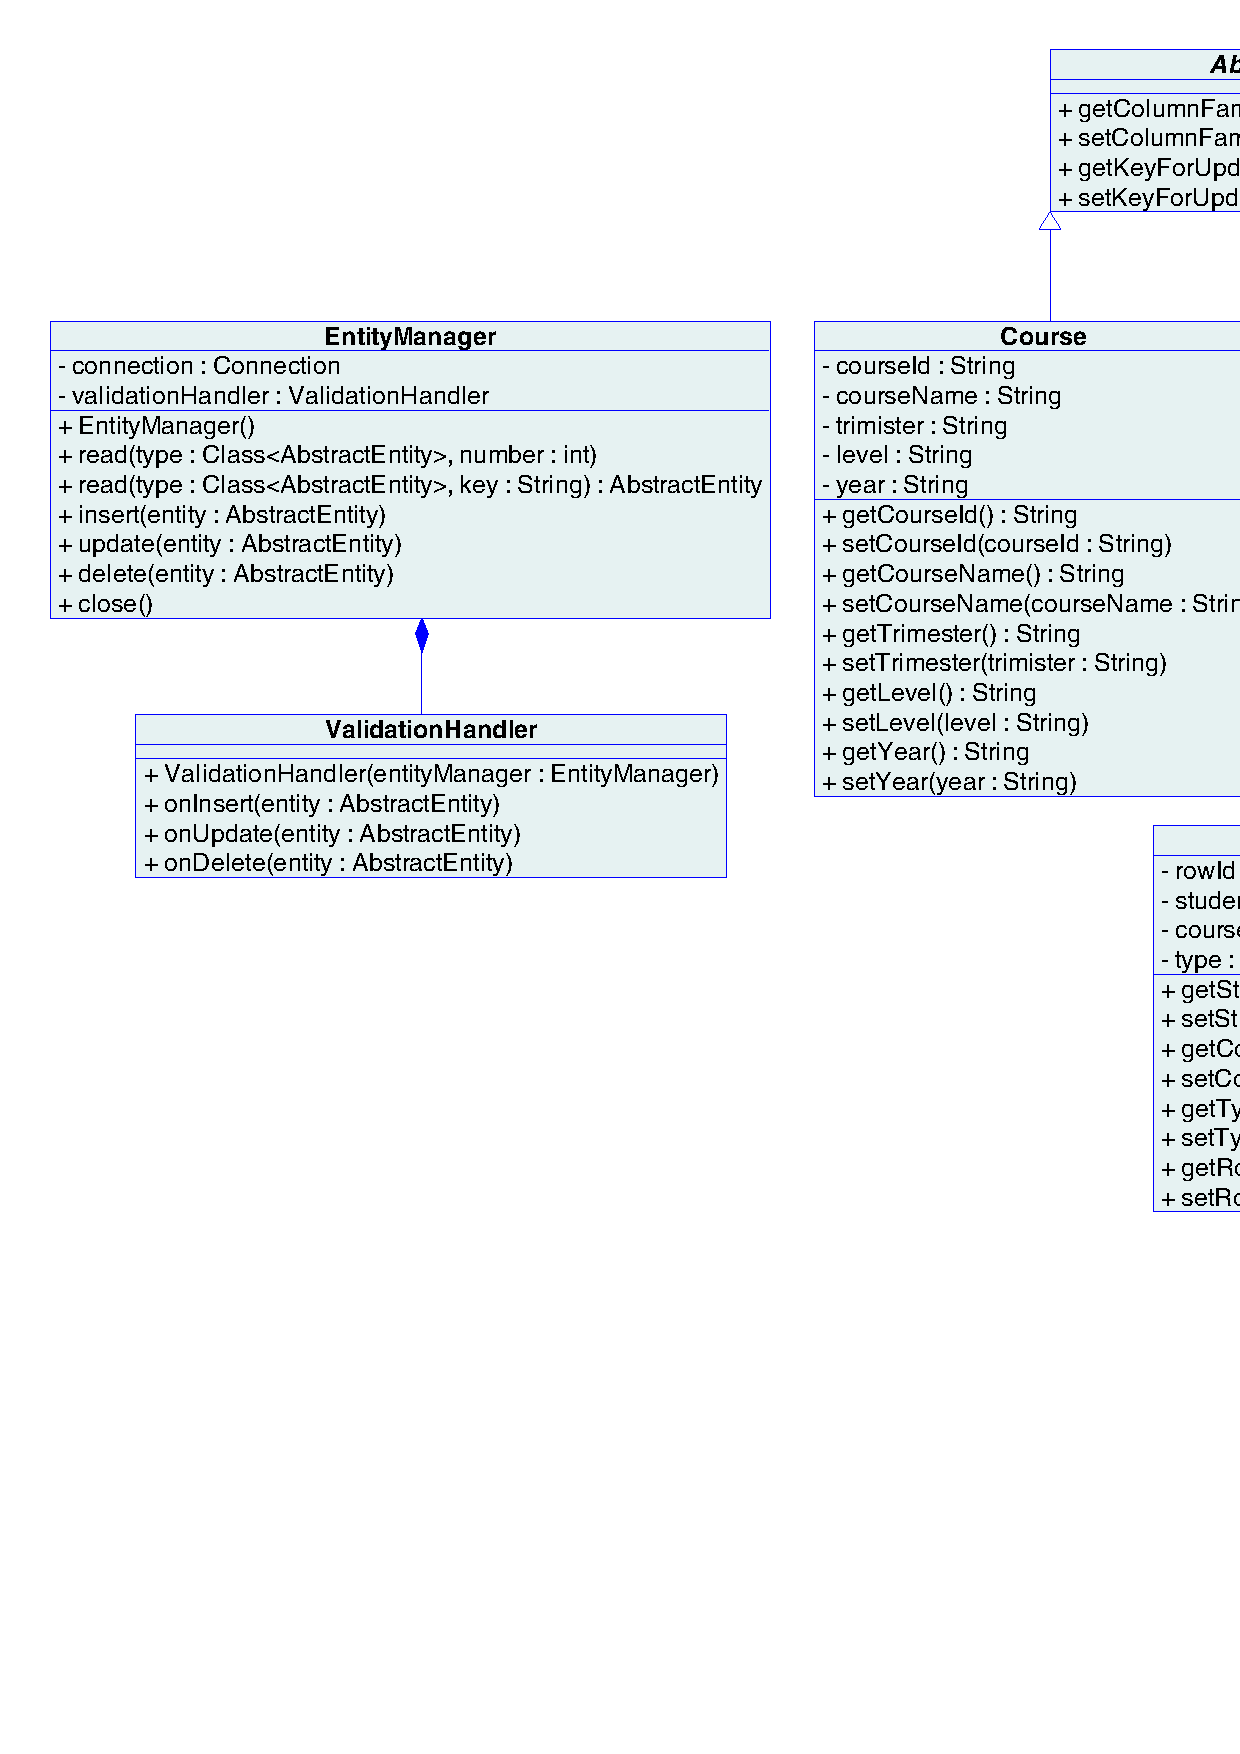
\includegraphics[width=\textwidth]{./figure/Solutions/FinalClassDiagram.png}
	\caption{Class Diagram for the \ac{API}}\label{f:classDiagram}
\end{figure}
% \end{landscape}

	\subsection{Entities} 
% 	An entity represents a real world object which has attributes
% 	associated with it and it is defined during the conceptual data modeling of
% 	data as in the popular \ac{ER} model(\todo{cite navathe}).
	An entity class contains attributes and their respective  getters and setters.
	 It represents a column family where each attribute is mapped into its
	 respective columns.  For example,  in the University keyspace , 
	\texttt{Enrolment} is an entity class that is mapped as the
	\texttt{Enrolment} column family and it contains the attributes RowId,
	CourseId and StudentId  mapped as its respective columns. Hence, an instance of
	\texttt{Enrolment} contains the values of one super column. Likewise, 
	\texttt{Student} and \texttt{Course} entities  map respective super columns in
	their column families.
% 	 The columns
% 	in the column family can be considered as the attributes of the entity instances. Some
% 	of the other entities for this example are \texttt{Course} and
% 	\texttt{Enrolment}.
	
	For all the solutions in this \ac{API},  entities of the user applications are
	designed to extend the abstract class called \texttt{AbstractEntity},  which has
	information about the  methods for accessing and defining  entities.  For
	every column family, applications derive a class from the
	\texttt{AbstractEntity} containing attributes.
	The \ac{CRUD} operations that can be performed on these entities like   are
	handled by the \texttt{EntityManager},  which is described in the following
	subsection.
		
	\subsection{EntityManager}
% 	Generally,  when any application connects to a database a session is maintained
% 	while this connection lasts.  During such sessions, applications
% 	maintain a persistence context, which is a cache to store the state information
% 	of entities retrieved from the database,  so that the database is not directly
% 	accessed for every operation on an entity (\todo{apachetomee,  javadoc}). 
% 	Commonly, the persistence context is accessed through an interface called
% 	\texttt{EntityManager} that provides the basic \ac{CRUD}
% 	operations to access entities.  Such an approach is adopted by this
% 	\ac{API} as well, where the \texttt{EntityManager} is called \texttt{EntityManager}.  
% 	
% 	However,  it
% 	is complex and computationally expensive to maintain such a persistence context
% 	for applications using cloud \acp{DBMS}, since entities are replicated on many
% 	nodes with the possibility of many users concurrently accessing and changing its
% 	state.  In such a dynamic environment,  maintaining the persistence context
% 	becomes an overload for applications, as it has to
% 	 connect to the underlying \ac{DBMS} often and ensure that the entities are
% 	 always up to date. 

	An \texttt{EntityManager} is in charge of performing all the \ac{CRUD}
	operations on the entities. To perform these
	operations  the \texttt{EntityManager}
	accesses a column family in the keyspace. It establishes a connection
	to a Cassandra cluster using Hector, which is one of the 
	 early Cassandra client \acp{API}.  Hector is a high level
	client that wraps the driver-level interface of Cassandra called Thrift and
	provides more benefits than Thrift like fail-over mechanisms and connection
	pooling (\todo{cite book}).  Hector was the preffered \ac{API} for this thesis
	since it encapsulates the interaction with the Thrift \ac{API} and makes it
	simpler to access a Cassandra cluster.
	% The learning curve to understand and use Thrift
	% proved to be steep and time consuming,  considering the scope of the thesis.
	% Hector was the chosen \ac{API} for this thesis since  it  abstracts the complex
	% interaction with Thrift and makes it easy to access a Cassandra cluster.
			
	The \texttt{EntityManager} creates a connection object
	using Hector's  connection manager to connect to a keyspace and this connection
	is used for all the operations on the entities.  For all the operations,
	it creates a \texttt{Mutator} object defined by Hector,  to
	insert,  update or delete an entity in the Cassandra cluster. The
	\texttt{EntityManager} provides the \texttt{Mutator} object with the entity
	details like its key, column family details. To extract  information
	from any entity during runtime, the \ac{API} uses reflection. This allows
	the \ac{API} to invole appropriate access methods from the entity class to
	retrieve the entity's information.
	Thus, this \ac{API} can be used for any application.
% In other
% words, the \texttt{EntityManager} connects to the keyspace directly and  accesses it by connecting to one of the nodes in
% the cluster for performing the operations on the entities.
% 	
	The \ac{CRUD} operations trigger  referential
	integrity validation on entities and to
	perform these validations the \texttt{EntityManager} passes the
	entity and the connection details to the \texttt{ValidationHandler},
	which is explained in Section~\ref{ss:VH}.
	The implementation of the \ac{CRUD} operations in the \ac{API} are described
	below.
% 	The validation is performed by the
% 	\texttt{ValidationHandler} which is explained in Section~\ref{ss:VH}. The
% 	\texttt{EntityManager} passes the entity and the connection details to the
% 	\texttt{ValidationHandler} for this. 
	
% 	The \texttt{EntityManager} uses refelection to extract information from any
% 	entity during runtime. 
% 	
	   % 
	% An
	% \texttt{EntityManager}
% 	represents the session an application maintains with the database.  It is
% 	basically the interface to access and interact with the persistence context, 
% 	which in simple terms is the cache of data retreived from the database.   Such a
% 	persistence  context helps as the numebr of times a database has to be directly
% 	accessed is reduced and instead a copy of the data persists in the memory and is
% 	used in the necessary operations required by the application,  thus recuding the
% 	consumption of many resources. This persistence context has a set of entity
% 	instances along with a set of operations to interact with these instances of
% 	data. 
		
% 	Generally,  applications that handle data in a database use an
% 	\texttt{EntityManager} to access the underlying database,  which performs the
% 	correct operations on the entities in the persistance context and these
% 	operations are commited into the database once a transaction is committed.  
%  	.  
 	 
	
		\subsubsection{Create}
		 The \texttt{create} operation stores entities in the respective column
		families. The \texttt{create} operation is also known as the
		\texttt{insert} operation. The \texttt{EntityManager} inserts these entities
		into the column families represented by the entity class.  
		For example,  all the student entities are inserted into the column family
		\texttt{Student} through the \texttt{EntityManager}. 
		
		While inserting entities,  Hector methods \texttt{createStringColumn()}, 
		\texttt{createKeyspace} and others are used by the \texttt{EntityManager} to
		create columns and keyspaces to insert the entities. The
		\texttt{EntityManager} passes the entity details which include entity key and
		column family information to \texttt{addInsertion} method of the \texttt{Mutator}.
		
% An \texttt{insert} operation inserts an entity into the database and commits
% it. 
		 The \texttt{insert} operation triggers a referential integrity
		validation whenever a child entity is  inserted in order to ensure that its
		parent entities exist. The validation is performed by the \texttt{onInsert}
		method of \texttt{ValidationHandler}, which is explained in
		Section~\ref{ss:VH}.
% 		Based on the referential integrity \texttt{insert} rule,   valid parent entities
% 		with primary keys matching the foreign keys of the child entities must exist , 
% 		else an exception is raised stating that the
% 		referential integrity has been violated.  
% 		The implementation of the \texttt{insert} operation is consistent across all
% 		the solutions. 
		
		
% 		The user application provides the metadata pertaining to their keyspace and
% 		this is inserted using this \texttt{insert}operation through the \texttt{EntityManager} in
% 		all the solutions. 
% This
% 		metadata also contains the data manipulation rule applicable for each entity, 
% 		like \texttt{Cascade} or \texttt{NoDelete}.  This is necessary for the
% 		\texttt{Update} and \texttt{Delete} operations. 
		
		\subsubsection{Read}
		In a \texttt{read} operation  entities are  retrieved by providing the
		entity class and its key. This operation does not prompt any referential integrity
		validation since entities are only read and their state is not changed, 
		 unlike in the other operations. 
% 		Every time entities are inserted,  updated or deleted,  the \texttt{read} operation is
% 		initiated by the \texttt{EntityManager} to retrieve the correct entities on which
% 		these operations are to be executed. 
		The key of the entity  that has to be read are passed from the
		solutions to the \texttt{EntityManager} and it in turns retrieves these entity
		instances (or the relevant super columns) from the column families.  This
		\ac{API} provides two \texttt{read} operations to retrieve a set of
		entities from an entity class or just a single entity by providing its key.
		
		
		\subsubsection{Update}\label{ss:update}
		In an \texttt{update} operation the existing state of an entity is merged
		with a new state. 
		This means that  values of columns are updated to new values and
		 committed into the column families by the \texttt{EntityManager}.  The
		\texttt{EntityManager} receives the entity and the new values provided by the user
		application and commits the changes to the column family of the entity. 
		
		Whenever an entity is updated, the \texttt{EntityManager} deletes the
		previous instance of this entity from its respective column family and inserts
		the entity with its new state into its column family.
		The \texttt{EntityManager} invokes  the \texttt{delete} operation to remove
		the old state and then invokes the \texttt{insert} operation to insert the new
		state of the entity.
		
		In all the solutions,  an \texttt{Update} operation triggers a referential
		integrity validation whenever any primary or foreign keys of any entities are updated.
		The validations are performed by the \texttt{onUpdate} method of the
		\texttt{ValidationHandler}.
		
		Whenever a primary key is updated to a new value, the
		\texttt{EntityManager} performs a few additional operations. It passes the entity to the
		\texttt{ValidationHandler} for referential integrity validation and receives
		the list of child entities if dependencies on this primary key exist. The
		following steps are performed after this :
		\begin{enumerate}
		  \item Store the list of child entities received from
		  \texttt{ValidationHandler} as a \texttt{List <E>} in
		  \texttt{EntityManager}.
		  \item Perform \texttt{delete} on the child entities from their column family
		  in Cassandra.
		  \item Perform a \texttt{delete} on the entity with the primary key from the
		  column family.
		  \item Perform an \texttt{insert} with the entity and its new primary key.
		  \item Update the foreign keys in \texttt{List <E>} of child dependencies to
		  the new value.
		  \item Perform an \texttt{insert} to insert the child entities into its
		  respective column family.
		\end{enumerate}
		
		These additional \texttt{insert} and \texttt{delete} operations are essential
		to overcome the tombstone delete performed by Cassandra which prevents
		changing a primary key (also called the row key).
% 		When a parent entity is updated on its primary key column,   the
% 		\texttt{EntityManager} checks the metadata to locate  any existing constraints on
% 		this parent entity.  If dependencies are found then,  based on the parent
% 		entity's \texttt{DeleteRule},  the child entities are either updated or the
% 		operation is cancelled.  If the \texttt{DeleteRule}  is \texttt{Cascade},  or
% 		is \texttt{NoDelete} but has no current child dependencies,  then the child 
% 		entities are correctly updated, prior to updating the parent entity's primary
% 		key column.  If the \texttt{DeleteRule} is \texttt{NoDelete},  with existing
% 		child dependencies,  the \texttt{update} operation is prevented and an
% 		exception is raised.  For example,  in the University keyspace example,  when a
% 		new \texttt{StudentId} is provided for an existing  \texttt{Student}
% 		instance in \texttt{Student} column family,  then \texttt{EntityManager} checks
% 		metadata and locates the \ac{FK} constraint \texttt{CONST400} as seen in
% 		Figure~\ref{f:meta-fk}, which shows the existing constraint on
% 		\texttt{Student}.
% 		Since the \texttt{DeleteRule} is \texttt{Cascade}, 
% 		all the old \texttt{StudentId} values for this \texttt{Student} 
% 		instance in \texttt{Enrolment} are updated with the new
% 		\texttt{StudentId} values, prior to updating the \texttt{Student} instance in
% 		the \texttt{Student} column family.
% 		
% 		When a child entity is updated on any of its
% 		foreign key columns,  the \texttt{EntityManager} performs the same check on the
% 		metadata and locates its parent entities and the referenced primary key columns. 
% 		If the new values of the foreign keys are not present as a primary key for any of the
% 		parent entity instances,   an exception is raised and this update is
% 		prevented, else  the update is performed.  For example,  when the foreign key
% 		\texttt{StudentId} for one of the instances in \texttt{Enrolment} is given a new
% 		value,  then the \texttt{EntityManager} identifies the parent entity for this
% 		\ac{FK} constraint as \texttt{Student}.  If the new
% 		\texttt{StudentId} exists as a primary key for any of the \texttt{Student}
% 		entities,  the \texttt{update} is performed. 
		
% 		To locate the references in the metadata as well as locating the correct
% 		entities and its columns,  the \texttt{BasDAO} performs the \texttt{Read}
% 		operations. 
% 		The \texttt{EntityManager} reads the metadata, the entities and its keys using
% 		the \texttt{read} operation. 
		
		\subsubsection{Delete}\label{ss:delete}
		In a  \texttt{Delete} operation, entities are removed from a column
		family. The \texttt{EntityManager} passes the entity
		information to the \texttt{delete} method of the \texttt{Mutator} object.
		
		In all the solutions,  a \texttt{Delete} operation triggers a referential
		integrity validation every time a parent entity is deleted. This validation is performed by
 		the \texttt{onDelete} method of the \texttt{ValidatinHandler}.
		% To validate referential integrity, the
% 		\texttt{EntityManager} performs a \texttt{read} operation on the metadata and locates  any existing \ac{FK} constraints that depends on the
% 		entity's primary key. 
% 		
% 		If the parent  entity has a \texttt{Cascade} rule,  or has a
% 		\texttt{NoDelete} rule with no current dependencies,  then the child entities
% 		are deleted prior to deleting the parent entity. 
% 		
% 		For example,  in the University keyspace,  if a 
% 		\texttt{Student} instance is marked for deletion,  then the \texttt{EntityManager}
% 		locates the child entities that are referencing \texttt{Student} like
% 		\texttt{Enrolment} from the constraint \texttt{CONST400}
% 		(Figure~\ref{f:meta-fk}).  Since the \texttt{DeleteRule} is \texttt{Cascade}, 
% 		the child entities are deleted from \texttt{Enrolment} prior to deleting the
% 		\texttt{Student} instance. 
		
		\subsection{ValidationHandler}\label{ss:VH}
		The \texttt{ValidationHandler} is invoked by the \texttt{EntityManager} every time
		an operation triggers a
		referential integrity validation on any entity. 
		The \texttt{EntityManager} passes the entity,  the connection details and its
		metadata to the \texttt{ValidationHandler} to perform the validation.  
		
		The \texttt{ValidationHandler} contains the logic for checking whether an entity
		has any dependencies and verifies whether an \texttt{insert}, \texttt{update} or
		\texttt{delete} operation  violates the referential integrity or not.
		To ensure that these operations maintain referential integrity between entities,
		it applies the appropriate referential integrity rules, as explained in
		Section~\ref{s:referential-integrity}. Thus, for an \texttt{insert} operation
		the insert rule of referential integrity is followed and similarly for
		\texttt{update} and \texttt{delete} operations their respective rules are
		applied.As previously mentioned, a \texttt{read} operation does not invoke any
		refreential integrity validation in this \ac{API}. The referential
		integrity validation performed by \texttt{ValidationHandler} for each of these
		operations is discussed next with pseudocodes.
		
		\begin{description}
		\item[onInsert]: 
		In an \texttt{insert} operation a referential
		integrity validation is triggered whenever a child entity is  inserted. 
		The \texttt{ValidationHandler} applies the referential integrity insert
		rule which checks whether  valid parent entities with
		primary keys matching the foreign keys of the child entities exist , else an
		exception is raised stating that the referential integrity has been violated.
		The implementation of the \texttt{insert} operation is consistent across all the
		solutions. 
		\todo{Insert Pseudocode}
		
		\item[onUpdate:] The validation for an \texttt{update} operation is different
		when primary keys and foreign keys are updated. 
		\begin{description}
		\item[Case A: Update Primary Key] When a  primary key of a
		parent entity is updated, the \texttt{ValidationHandler} performs the
		following checks.
		\renewcommand{\labelenumii}{\arabic{enumi}.\arabic{enumii}}
		\renewcommand{\labelenumiii}{\arabic{enumi}.\arabic{enumii}.\arabic{enumiii}}
		%\renewcommand{\labelenumiiii}{\arabic{enumi}.\arabic{enumii}.\arabic{enumiii}.\arabic{enumiiii}}
		\begin{enumerate}
		  \item if \ac{FK} constraints on primary key exist
		  	\begin{enumerate}		  	
		    \item if \texttt{DeleteRule} for the \ac{FK} constraint is
		    \texttt{Cascade}
		    	\begin{enumerate}
		    	  \item Pass any existing child entities to the \texttt{EntityManager} to
		    	  allow update of both parent and child entities.
				\end{enumerate}
			\item else if \texttt{DeleteRule}  is \texttt{NoDelete}
				\begin{enumerate}
				  \item if no child entities exist
				  		\begin{enumerate}
				  		  \item \texttt{EntityManager} performs update on  the primary key
				  		\end{enumerate}
				  \item else if child entities exist
				   		\begin{enumerate}
				    	\item Raise exception and rollback \texttt{update}. 
				    	\end{enumerate}
				\end{enumerate}
			\end{enumerate}
		  \item else if no \ac{FK} constraints are found 
		  		\begin{enumerate}
		  		  \item \texttt{EntityManager}
		  performs update on the primary key
				\end{enumerate}
		 \end{enumerate}
		 
% 		 checks the metadata to locate any existing \ac{FK} constraints on
% 		this parent entity.  If dependencies are found then,  it verifies the parent entities
% 		\texttt{DeleteRule}. The \texttt{EntityMananger} is informed that the 
% 		child entities can be updated if the \texttt{DeleteRule} is
% 		\texttt{Cascade} else the \texttt{update} operation is cancelled and an exception raised.
% 		 Another case where the \texttt{update} operation is performde is when the
% 		\texttt{DeleteRule} is \texttt{NoDelete} but there are no existing \ac{FK}
% 		constraints.
		
% 		If the \texttt{DeleteRule}  is \texttt{Cascade},    then the child entities 
% 		are correctly updated, prior to updating the parent entity's primary key column.  
% 		If the \texttt{DeleteRule} is \texttt{NoDelete},  with existing
% 		child dependencies,  the \texttt{update} operation is prevented and an
% 		exception is raised. 
		For example,  in the University keyspace,  when a
		new \texttt{StudentId} is provided for an existing  \texttt{Student}
		entity in the \texttt{Student} column family,  then \texttt{ValidatinHandler}
		checks metadata and locates the \ac{FK} constraint \texttt{CONST400} as seen in
		Figure~\ref{f:metadataInSolutions}. Since the \texttt{DeleteRule} is
		\texttt{Cascade}, the \texttt{EntityManager} allows the \texttt{update}
		operation to take place.
% 		all the old \texttt{StudentId} values in \texttt{Enrolment} are 
% 		updated with the new
% 		\texttt{StudentId} values, prior to updating the \texttt{Student} instance in
% 		the \texttt{Student} column family.
		
		\item[Case B: Update Foreign Key] When a foreign key of a child entity is
		updated , the\newline  \texttt{EntityManager} performs the same check on the
		metadata and locates its parent entities. It then follows these steps:
		\begin{enumerate}
		  \item Identify parent entity class from the \ac{FK} constraint
		  \item if new foreign keys exist as primary keys in parent entity class
			\begin{enumerate}
				\item \texttt{EntityManager} updates  the foreign key
			\end{enumerate}
		  \item else 
			\begin{enumerate}
				\item Raise exception
			\end{enumerate}
		\end{enumerate}

% 		If the new values of the foreign keys are not present as a primary key for any
% 		of the parent entity instances,   an exception is raised and this update is
% 		prevented, else  the update is performed.  
		For example, when the foreign key \texttt{StudentId} for one of the entities
		in \texttt{Enrolment} is given a new value,  then the \texttt{ValidationHandler} 
		identifies the parent entity class for its \ac{FK} constraint
		\texttt{CONST400} as \texttt{Student}.  If the new \texttt{StudentId} 
		exists as a primary key for any
		 of the  entities in \texttt{Student} entity class,  the \texttt{update} is
		 performed.
		
		\end{description}
		The implementation of the \texttt{update} operation for both the cases is
		consistent for all solutions.
		
		\item[onDelete:]To validate referential integrity, the \texttt{EntityManager}
		performs a \texttt{read} operation on the metadata and locates  any existing
		\ac{FK} constraints that depends on the entity's primary key.
		
		If the parent  entity has a \texttt{Cascade} rule,  or has a
		\texttt{NoDelete} rule with no current dependencies,  then the child entities
		are deleted prior to deleting the parent entity. 
		
		For example,  in the University keyspace,  if a 
		\texttt{Student} instance is marked for deletion,  then the \texttt{EntityManager}
		locates the child entities that are referencing \texttt{Student} like
		\texttt{Enrolment} from the constraint \texttt{CONST400}
		(Figure~\ref{f:meta-fk}).  Since the \texttt{DeleteRule} is \texttt{Cascade}, 
		the child entities are deleted from \texttt{Enrolment} prior to deleting the
		\texttt{Student} instance. 
		\end{description}
		
		
		Since metadata is stored differently in the solutions , the
		\texttt{ValidationHandler} is different for each solution in the \ac{API}.For
		example,  the \texttt{ValidationHandler} for Solution 1 and 2 involves parsing
		the metadata since it is stored as a \texttt{String} along with the actual data.
		
		For example,  in the University keyspace, if
		the new foreign key \texttt{StudentId} for an \texttt{Enrolment} entity
		instance does not exist as a primary key for any of the \texttt{Student}
		instances in \texttt{Student},   the \texttt{ValidationHandler} signals
		\texttt{EntityManager} to raise an exception and to abort the operation.  The	pseudocode for validating the referential
		integrity in an \texttt{Update} operation is shown in
		Figure~\ref{f:VHpseudocode}. 
		(\todo{Change to text later}) \begin{figure}[h]
			\centering
			%\includegraphics[width=5cm,    height=5cm]{.  /figure/random.  jpg}
			\includegraphics[width=.8\textwidth]{./figure/Solutions/VH-UpdatePseudocode.png}
			\caption{\texttt{ValidationHandler} Pseudocode for an
			\texttt{Update} operation}\label{f:VHpseudocode}
		\end{figure}
		
		  
		
		
		
% 		\subsection{Connection to Cassandra}
% 		In the experimental \ac{API}, to perform an operation on entities a column
% 		family belonging to a keyspace in Cassandra cluster has to be accessed. The
% 		experimental \ac{API} establishes a connection to a Cassandra cluster,  using
% 		one of the early Cassandra client \acp{API},  Hector.  Hector is a high level
% 		client that wraps the driver-level interface of Cassandra called Thrift and
% 		provides more benefits than Thrift like fail-over mechanisms and connection
% 		pooling (\todo{cite book}).    The learning curve to understand and use Thrift
% 		proved to be steep and time consuming,  considering the scope of the thesis.
% 		Hector was the chosen \ac{API} for this thesis since  it  abstracts the
% 		complex interaction with Thrift and makes it easy to access a Cassandra
% 		cluster.
% 		
% 		To connect to a keyspace,  \texttt{EntityManager} creates a connection object for
% 		each of the solutions using Hector's  connection manager and this connection
% 		is used for all the operations on the entities.  To perform all the \ac{CRUD}
% 		operations on the entities,  \texttt{EntityManager} connects to the keyspace and uses
% 		Hector's methods to commit these changes to Cassandra.  
		
% 		While inserting	entities,  Hector methods like \texttt{createStringColumn()}, 
% 		\texttt{createKeyspace} and so on are used by the \texttt{EntityManager} to create
% 		columns and keyspaces based on the data provided by the user
% 		applications.  For all the operations, \texttt{EntityManager} creates a
% 		\texttt{Mutator} object defined by Hector,  to insert,  update or delete an entity in the
% 		Cassandra cluster.  For example,  in an \texttt{insert} operation, 
% 		\texttt{EntityManager} passes the entity details like its key and column family
% 		information to \texttt{addInsertion} method of the \texttt{Mutator}.
		% Similarly, \texttt{delete} method of \texttt{Mutator} is used for
		% \texttt{EntityManager's} \texttt{delete} operations.
		
		The implementation,  connection settings and operations using
		Hector methods are common for all the solutions in the \ac{API}.  
		The following sections describe the solutions,  the motivation for the
		solution's design and the way the solutions save metadata. 
		
% 	,  except that all the operations
% 	are directly sent to the database through one of the \acp{API} provided by
% 	Cassandra.  This is because  Cassandra does not perform transactions as seen in
% 	\acp{RDBMS},  but rather operations on data at a time (\todo{cite}). 
% 	\texttt{EntityManager} 
	
\section{Solution 1:  Metadata with Special Characters}\label{s:sol1}
% In RDBMSs,  referential integrity constraints are enforced at the creation of
% tables (or updated later using ALTER TABLE).  In the above example,  imposing
% the referential integrity constraint for the Enrolment table (Figure 3) would
% be using "FOREIGN KEY CourseID REFERENCES Course (CourseID)".  This would
% indicate that the CourseID of Enrolment table is dependant on the CourseID
% primary key of the Course table. 
	Much research has been done in the area of  metadata management in distributed
	environments,  where emphasis is laid on the synchronous updates of metadata
	storage as well as its efficient storage and access mechanisms(\todo{cite more}
	Hackl et al.  2010). 
	In Hackl et al.  (2010),  metadata management is discussed in the context of
	huge file systems, where metadata is stored separately in a suitable \ac{DBMS}
	so that such file systems can be managed and administered efficiently without
	slowing them down.  To analyse which type of \ac{DBMS} was more suitable for such a
	metadata storage,  they conducted various experiments and concluded that
	key-value \acp{DBMS} were more efficient in terms of speed,  memory and resource
	consumption when compared to popular \acp{RDBMS}.  As a part of their
	experiments, they adopted an interesting approach to store metadata in a
	key-value \ac{DBMS} ,  namely Tokyo Cabinet,  a popular \ac{NoSQL} \ac{DBMS}
	that stores records as simple key-value pairs in data files. Unlike Cassandra,
	tokyoCabinet does not involve data types or columns
	and so on (\todo{cite}).  In their approach,  metadata about the file system
	used in their experiment is inserted as a value which is associated with a unique key and the
	different parts of the metadata are separated by semicolons (Hackl et al.  2010). 
	
	The first solution   in this thesis is inspired by this design of saving
	metadata as the value in a key-value pair  in
	column-oriented key-value \acp{DBMS} . 
	The solution proposes saving the dependency information of the entities as
	metadata and including it in the entity's value.  In this solution, the 
	different parts of the metadata like \texttt{ConstraintName},  \texttt{RColumn},  \texttt{RConstraintName} and so on
	are separated by a special character like a comma. 
	To achieve this in a column-oriented key-value \ac{DBMS}, the metadata is saved
	as a part of each of the super column (or row) in a column family. 
	In every super column,  this metadata is separated from its columns
	 by storing the metadata surrounded with curly brackets. For example,  in the
	 University keyspace example,  the column family of \texttt{Student} would save
	 the dependency information as a part of the value  for every  super
	 column in it (Figure~\ref{}). 
	
	For this solution,  the metadata is
	parsed by the \texttt{ValidationHandler} and  the different parts of the
	metadata are extracted to identify whether the entity has any dependencies.   
	Each constraint in the metadata is handled as a
	\texttt{String} and the special characters like '\texttt{\{}',  '\texttt{, }'
	become the delimiters for parsing the \texttt{String} and splitting it into tokens.  
	Thus,  each of these tokens
	would hold one of the parts of the constraint like \texttt{RColumn}, 
	\texttt{DeleteRule} and so on. 
	When foreign key relationships are found by the
	\texttt{ValidationHandler}, after parsing the metadata for an entity,  the
	appropriate actions are triggered like throwing an exception thus preventing the operation 
	or allowing the operation to execute. 
	
	In this solution, the metadata is saved  when entities are inserted into the
	column family and thus the metadata is a part of each of the entity.  Since the
	metadata is present as the value in every super column,  accessing the metadata
	information for referential integrity validation is as simple as accessing the
	value itself,  requiring no additional actions or connection to the
	keyspace. Saving the metadata as embedded metadata in this solution is useful
	as entities are replicated across the distributed cluster, making metadata
	easily accessible by every node in the cluster, since it is a part of the
	entity.
	The \ac{API} parses the metadata of an entity by reading any of its instances
	and need not load metadata from any external location.
	
	On the other hand,  the metadata for an entity would be the same for all its
	instances .  For example,  in the University example,  the metadata
	information for the \texttt{Student} entity is applicable to each of its
	instances,  indicating that each instance  should have a primary key called
	\texttt{StudentID}. 
	Similarly,  all \texttt{Course} instances have the same \ac{PK} constraints
	applied on it.  When metadata is saved as a part of the  value, 
	every instance of an entity will contain the constraint information
	in it's value.  Since the metadata information and constraints are same for all
	the instances of a single entity ,  this metadata is repeated every time an
	instance of the entity is inserted.  For example,  if 
	\texttt{1000} \texttt{Student} instances are inserted,  the metadata for these
	\texttt{1000} instances are saved \texttt{1000} times too, along with these
	instances.  But the metadata is exactly same for all the
	instances \todo{(Figure~\ref{})}. 
	
	
	The distributed nature of cloud \ac{NoSQL} \acp{DBMS} also means that the
	metadata is not only repeated several times within the same column family,  but
	also across the nodes in the cluster, thus increasing the redundancy of
	the metadata.  But such a redundancy and consumption
	of space to store the metadata is not a potential issue 
	in cloud column-oriented key-value \acp{DBMS}, since storage on the cloud is
	inexpensive and  does not affect the economic benefits.
	
	Such a storage mechanism is not expected to affect the efficiency of the
	cluster negatively as the metadata information is not large in size and is
	easily replicated along with the actual data and does not exert any extra
	resources in the cluster.  The performance of this solution is analysed  in
	Chapter~\ref{}. 
	
	
	
\section{Solution 2:  Metadata as Top Row}\label{s:sol2}



\section{Solution 3:  Metadata Tables}\label{s:sol3}



\section{Solution 4:  Metadata Clusters}\label{s:sol4}

\section{Limitations}\label{s:lim}
Transaction
cascade on one level of nesting
unique or composite keys
school network  -->  experimental design




